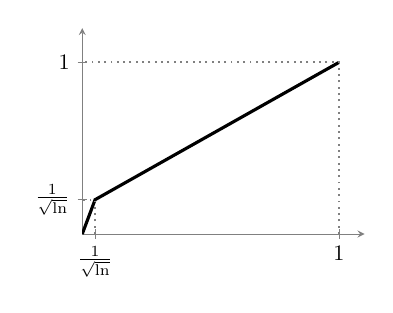
\begin{tikzpicture}[scale=0.8, transform shape]
\begin{axis}[
axis line style=gray,
axis lines=middle,
xlabel = $\quant$,
ylabel = $\revcurve$,
xtick={0, 0.05, 1},
ytick={0, 0.2, 1},
xticklabels={0, $\frac{1}{\constantH\sqrt{\ln\constantH}}$, 1},
yticklabels={0, $\frac{1}{\sqrt{\ln\constantH}}$, 1},
xmin=0,xmax=1.1,ymin=-0.0,ymax=1.2,
width=0.5\textwidth,
height=0.4\textwidth,
samples=1000]


\addplot[black!100!white, line width=0.5mm] (0, 0) -- (0.05, 0.2) -- (1, 1);


\addplot[dotted, gray, line width=0.3mm] (1, 0) -- (1, 1) -- (0, 1);
\addplot[dotted, gray, line width=0.3mm] (0.05, 0) -- (0.05,0.2) -- (0, 0.2);



\end{axis}

\end{tikzpicture}